% !TEX root = ../../main.tex

Edge computing enables a new class of distributed {cooperative}
applications.%
One example is a multiplayer game, where users and bots update a shared
game universe.
Other examples include users contributing to a cooperative document,
sharing files, using version control software, or a group of engineers
using augmented reality to design an artifact.
Maintenance engineers of a water-distribution company need data in the
field to access the pipes.
Telecom network engineers set systemwide configuration variables that
interact at remote devices.
Future applications might include vehicle-to-vehicle collaboration, or
informed tactical decision-making in an emergency.


Such applications are based on shared, persistent, mutable state, i.e.,
a database.
Whereas the database is stored centrally in a cloud setting, we enable
state to be distributed and replicated across decentralized edge
devices.
Locating data at the edge enables quick application response (no waiting
for a network round-trip) and availability (the application can read and
write data, even when disconnected from any remote server).
This local-first approach provides users with a sense of ownership and
helps with confidentiality \cite{rep:app:1827}.
Nonetheless, we leverage the strengths of the cloud infrastructure,
i.e., stronger consistency and well-managed, abundant resources.

Many distributed applications are currently designed to operate under strong consistency models, using solutions such as replicated state machines. This is due to the complexity of designing applications under weaker consistency models. Unfortunately, the use of these techniques is incompatible with the properties stated above. Therefore, there is a clear need to rethink how to develop distributed applications to work in edge computing environments.

It should be possible to execute in the cloud a computation that
requires high bandwidth (e.g., analytics) or stronger consistency.
The requirement is uniform semantics, i.e., wherever it executes, the
same computation observes the same state and has the same result; only
performance should differ.

\section{Consistency requirements}
\label{sec:consistency}
  
An edge application must remain available despite unpredictable network
connectivity, disconnection, and mobility.
Users or groups of users may have to work in isolation.
In this context, strong consistency is not possible globally
\cite{rep:pan:1628}.
  
One can argue that users are tolerant, and that a best-effort approach
such as Eventual Consistency (EC) is good enough.
This was the original approach for large-scale internet applications
such as e-commerce or social networks \cite{rep:syn:pan:1624}.
However, EC loses updates, which is clearly undesirable, e.g., in a
collaborative editing context.
  
Consistency anomalies are frustrating for users and make it difficult to write
a correct application code.
Thus, Facebook has moved to enforcing the read-your-writes guarantee
\cite{syn:1840}.
In networked video games, it frequently occurs that the user observes
an action, only to see the system roll it back soon afterwards
\cite{app:rep:1839}.
Applications, AIs, or decision-making software is more likely to have
bugs.
We take a hybrid approach: globally, provide the strongest model
compatible with availability; and locally, strengthen the guarantees
where possible.

\section{Global Consistency Guarantee: TCC+}
\label{sec:glob-cons-guar}

In the edge context, two different consistency models have been
explored.
Although they are incomparable, both have been proved to be a
strongest possible model compatible with availability under partition.

One is Monotonic Prefix Consistency (MPC), which combines the
per-process order into a global total order; however a process is
exposed to arbitrary rollbacks \cite{formel:syn:1806}.
We argue that a client losing an unpredictable amount of work is
an unacceptable user experience.

One is Monotonic Prefix Consistency (MPC) \cite{formel:syn:1806}.
In MPC, processes agree on a (monotonically growing) common prefix of
their individual sequential history.
In other words, MPC provides strong consistency up to the common
prefix, but recent history may diverge.
After applying some updates, a process might discover that another
update comes earlier in the sequential order, and have to roll back an
arbitrary number of times. MPC was the model of Bayou
\cite{syn:optim:rep:1433}, and lives on in blockchains
\cite{pass2017analysis, garay2015bitcoin} and in some recent file
systems \cite{syn:app:rep:1841}.
We argue that arbitrary rollback and loss of work are a poor user
experience, which is especially painful when nodes can disconnect for a
long duration.

Our preferred alternative is Causal Consistency (CC)
\cite{syn:rep:1738}.
Intuitively, if a client observes some update, it also observes all
preceding updates.
Only concurrent updates may be observed in different orders.

The following example illustrates ordering anomalies when CC is not
observed.
Alice makes her
photo album private, then adds a new photo. Later, Bob views Alice's
area. If the system does not enforce CC, he might see the new photo,
unless the website developer went to extra lengths to avoid this.
Instead, under CC such anomalies do not occur.

CC can be enforced locally and does not require consensus.
On top of CC, atomic transactions and convergence guarantees can be
supported without impacting availability
\cite{rep:pan:sh177,rep:pro:sh182}.
This improved model is called \emph{Transactional Causal Plus
  Consistency (TCC+)}.
Section~\ref{sec:tcc-guarantees} formalizes the TCC+ guarantees.
The drawback is that tracking the partial order in CC (and hence TCC+)
can have a heavy metadata cost, as we discuss later.

\section{Conflict-Free Programming}
\label{sec:requirements:conflict-free-programming}

We briefly introduce the main ideas of conflict-free programming and explain how they adapt to edge computing \cite{shapiro2011conflict, almeida2015efficient}. Traditional approaches to distributed system design are not generalizable to edge networks because they depend on strong synchronization between multiple parties, such as that provided by uniform consensus. Unfortunately, such strong synchronization primitives are impossible to realize in a scalable manner on edge networks. An alternative to using such primitives is to rely on conflict-free programming.

Consider a distributed data structure, replicated across \textit{n} nodes to improve robustness to node failures. Each node has a copy of the current value of the data structure. When an operation is invoked on a node, a new value is calculated and all nodes must be updated with this new value. This operation must be performed consistently in the event of concurrent operations, node failures, and network disruptions ranging from variable latency to message drop or partitions.

Relying on strong synchronization primitives, one would use a solution based on a uniform consensus algorithm such as Multi-Paxos \cite{chandra2007paxos} or Raft \cite{ongaro2014search}. Many industrial systems use this solution, for example, Google's Chubby lock service uses Multi-Paxos. In this solution, the consensus algorithm is run on all \textit{n} nodes for each operation, which, in addition to being expensive and not scalable, does not provide availability in the event of a major node failure or network disruption.

The alternative proposed in the context of conflict-free programming is based on the observation that, in most cases, consensus is not strictly necessary to maintain replicated data structures. Replicated data structures can be realized using a conflict-free replicated data type (CRDT) \cite{shapiro2011conflict}. A CRDT satisfies the mathematical property of Strong Eventual Consistency (SEC), which ensures that replicas are consistent as soon as they observe and execute the same set of operations.

This allows programming distributed applications that do not have to explicitly worry about synchronization between components that may be loosely coupled. Instead, it becomes sufficient to ensure that \textit{eventually} the different components of the system are able to communicate with each other and exchange synchronization information, which is much weaker than uniform consensus.

This approach works well and is used in several industry systems, such as applications from SoundCloud, Bet 365, Riot Games, Rovio and Trifork. And its success points to the need to further leverage synchronization-free programming models to develop robust and available applications within the edge-computing model.

\section{Local Strengthening: Data Center}
\label{sec:strength-guar}

A set of nodes that are strongly connected to each other can support
even stronger guarantees.
The system can totally order updates upfront, ensuring for instance
Snapshot Isolation (SI).
SI is stronger than MPC, as it does not suffer rollbacks, and than CC,
as it totally orders updates.
The metadata cost for total order is much reduced.
We call a set of nodes that enjoy SI among themselves an \emph{SI zone}.

One kind of SI zone is a single data center (DC).
A DC has a large number of parallel servers, connected through a
high-quality network.
\system{} executes transactions across multiple servers in the same DC
under SI
Snapshot Isolation (SI), an RFTOC model that is strictly stronger
than CC \cite{rep:pan:1723, rep:pro:sh182}.

\begin{figure}[tph]
  \centering
  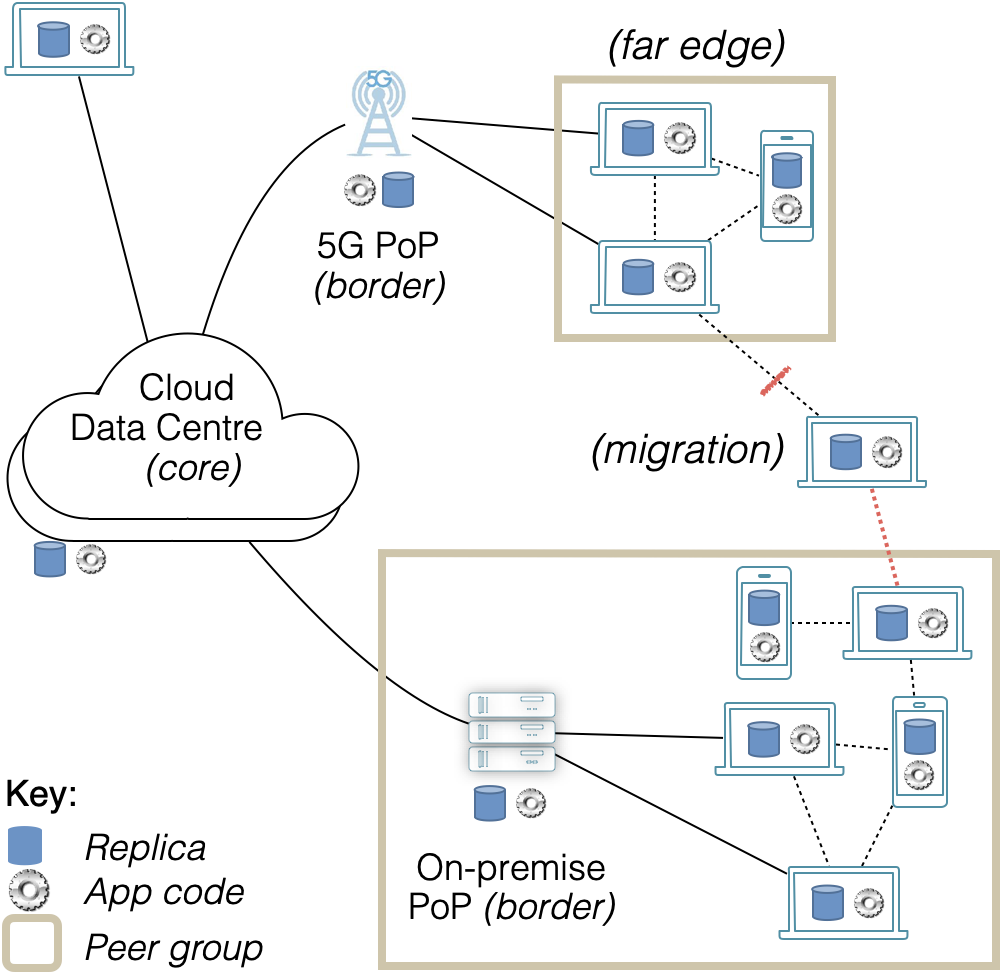
\includegraphics[width=0.8\textwidth]{figures/topology.png}
  \caption{
    Example \system{} topology.
    \protectA small number of DCs forms the core.  A far edge device connects either directly to a DC, or via a point-of-presence (PoP) server at the border.  A peer group contains devices in geographical proximity.  Note the device migrating between subtrees.
  }
  \label{fig:topology}
\end{figure}

In the context of global TCC+, a DC counts for a single sequential
process, thus limiting metadata size.

Some systems support two classes of transactions, weak and strong; all
transactions follow causal order, and in addition strong transactions
are globally totally ordered \cite{rep:syn:1690, rep:syn:1845, rep:syn:sh167}.
\system{} does not currently support strong operations, but does support
an intermediate class of ``moderate'' transactions that are totally
ordered within a peer group.

\section{Local Strengthening: Peer Groups}
\label{sec:node-grouping}

This section  examines another kind of SI zone, the peer group.
Inconsistency is especially problematic to users who communicate
directly, outside of the database.
For instance, in the enhanced-reality game Pokémon~Go, two users in
close proximity can both become the owner of the same game character
\cite{pokemon-go-anomaly}; this anomaly confuses the users.
Another case is a group of collaborators that wish to follow each other
closely, without receiving  distracting updates from the
outside.
This and similar examples argue for groups with stronger consistency.

There are different kinds of groups:
A \emph{collaboration group} is a set of nodes collaborating which each
other and separately from others.
Desirable features include branching versions, and security
mechanisms for managing trust.
The group may be short- or long-lived, and its nodes may be
geographically close or far away.

A {lateral group} is a set of nodes that communicate directly
with one another.
This enables them to remain independent, even if the cloud happens to be
unavailable.

The group is short-lived and lasts only as long as the lateral
connection.

An {SI zone} is a set of nodes that enforce strong consistency
locally, by leveraging  stable and low-latency network connection to
one another.
This kind of group is also short-lived.

For simplicity, in \system{} a lateral group is also an SI zone; we will
call this a \emph{peer group.}

In \system{}, edge nodes in network proximity can
constitute an SI zone, called a \emph{peer group}.
According to SI, transactions become visible in some \emph{a priori}
total order with no rollback.
This approach improves user experience and helps to manage metadata.

To avoid that these stronger guarantees be at the expense of
availability, the system should support disconnected work and mobility
within the topology, without losing the TCC+ guarantees.

For instance, users traveling together on a bus might create an SI
group to play a multi-user game together; as the bus moves away from
its connected DC, it can switch to a closer one.

\section{Security Requirements}
\label{sec:secur-requ}

A different concept is the \emph{collaboration group,} a set of nodes
that collaborate together, even when far from each other.
For this
case, 
To support collaboration, 
\system{} supports versioning and trust management.

Because it is the edge device that executes and merges updates, data can
remain encrypted end-to-end; the untrusted cloud serves merely for
transport and persistence \cite{sec:rep:1823}.

On the other hand, the edge use case poses new security challenges.
Information is exposed on compromised edge nodes \cite{syn:sec:1838};
security policy changes and data updates are concurrent
\cite{rep:sec:1692, sec:rep:1786}; and decentralized key management is
problematic \cite{sec:rep:1823}.
We alleviate these difficulties by leveraging the cloud, e.g., for
authentication and key management.

Our focus in the security area is on the management of mutual trust to
support group collaboration.
Every data object comes with an Access Control List (ACL) that describes
what updates different users are allowed on the object.
The system preventatively enforces ACL in edge devices.
Because an edge device may be compromised, every node double-checks the
updates it receives, and masks an update that is not allowed by the
corresponding ACL, and transitively any update that depends on it.
Thus a correct node never depends upon a state that violates the security
policy.

\section{Summary}
The ever-increasing amounts of data generated on the Internet pose real challenges to the cloud computing model that often delegates most of its computation and storage to the cloud data center. The Edge/Fog Computing model can be seen as a distributed extension of the cloud computing model by breaking down the core cloud into a network of smaller clouds (i.e., the Fog) often located close to the user, bringing several performance benefits and new classes of applications.

Many distributed applications are currently designed to operate under strong consistency models, using solutions such as replicated state machines. This is due to the complexity of designing applications under weaker consistency models. Unfortunately, the use of these techniques is incompatible with the properties stated above. Therefore, there is a clear need to rethink how to develop distributed applications to work in edge computing environments.
